\section{Pain}
Pain is defined, by the International Association for the Study of Pain, as an unpleasant sensory and emotional experience associated with actual or potential tissue damage~\cite{Kerstman2013}. 
Pain is a sudden or slow onset of any intensity from mild to severe pain~\cite{Mello2016} and can be categorized based on the pain experience as acute, chronic and intermittent pain~\cite{Goldberg2011}. Acute pain is anticipated or predictable, while  chronic pain is not anticipated or predictable. Chronic pain has a duration greater than three months with a constant or recurring of pain. Contrary to chronic pain, intermittent pain is not constant but has interruptions in between~\cite{Mello2016}.

Pain is a worldwide problem and affects all populations regardless of gender, age, income, ethnicity or geography. However, the distribution across the globe differs due to different risk factors such as female gender, injury and psychosocial environment \cite{Macfarlanea2016}.  The prevalence and incidence is high despite the complexity of quantifying pain. It is estimated that 20\% of the world's populations adults suffer from pain and each year 10 \% is diagnosed with chronic pain~\cite{Goldberg2011}. 

The frequently causes of pain are trauma, surgery, cancer, osteoarthritis and rheumatoid arthritis, injuries and spinal cord problems. Furthermore, pain can lead to different conditions, such as depression, inability to work, limited social relationships and suicidal thoughts.~\cite{Goldberg2011, Breivik2006}

People with chronic pain often complain of cognitive problems which interfere with their daily functions. Additionally, it is indicated that among people with chronic pain there is a consistent evidence for disturbances in attentional capacity, processing speed, and psychomotor speed. However, the relationship between pain and cognitive problems is unknown.~\cite{Geisser2018}

\subsection{Types of pain}
Pain can be divided into nociceptor pain and neuropathic pain~\cite{Steeds2013}. Nociceptor pain can be classified attending to the location of pain as somatic pain or visceral pain. Somatic pain occurs when nociceptors in skin, muscles, skeleton, joints or connective tissues are activated. Visceral pain is defined as pain that results from the activation of nociceptors in the thoracic, pelvic or abdominal viscera. Unlike somatic pain, visceral pain is harder to localize within the body. Another type of pain is neuropathic pain, which is caused by a primary lesion or dysfunction of the peripheral nervous system or central nervous system. The main difference from nociceptor pain is that neuropathic pain has an absence of continuous nociceptive inputs. \cite{Kerstman2013}

\subsubsection{Nociceptor pain}
Nociceptors are free nerve endings and have a high threshold for mechanical, chemical or thermal stimulation. There are two types of nociceptors, $\alpha\delta$ and C fibers. $A\delta$ fibers are myelinated nerve cells with a diameter between 2 and 5$\mu$m, which produce fast well localized sharp pain. Those fibers are mostly distributed in the body surface, muscles and joints. C fibers are unmyelinated nerve cells with a diameter below 2$\mu$m, which produce slow and poorly localized burning and throbbing pain. The C fibers are distributed in most tissues. \cite{Steeds2013}

When a noxious stimulation occurs, the nociceptors will be activated and propagate the pain information to the spinal cord via dorsal horn, which is illustrated as the red arrow on \figref{fig:pathways}~\cite{Martini2012}. The second order neuron is activated by the release of neurotransmitters from the nociceptor. The second order neuron receive these information and cross over to the opposite side of the spinal cord and brings the information towards the brain via the lateral spinothalamic tract, which is indicated by the white arrow on \figref{fig:pathways}. This information will be transmitted by releasing neurotransmitters to the third order neuron in the thalamus. The third order neuron localizes and discriminates the pain in the brain, illustrated as a black arrow on~\figref{fig:pathways}, but in the opposite side from where the pain actually occurred. Perception of pain on the right side of the body is processed on the left side of the brain and vice versa~\cite{Martini2012}. 


\begin{figure}[H]
	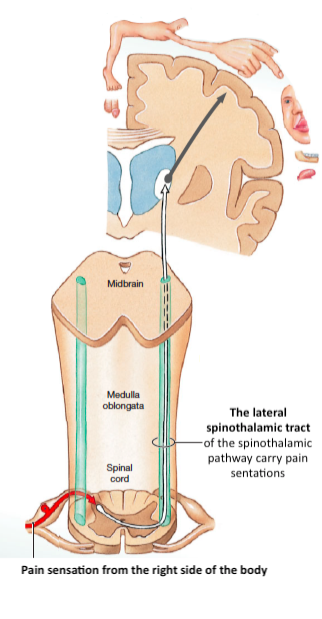
\includegraphics[width=0.5\textwidth]{figures/pathways.png} 
	\caption{Spinothalamic pathway. Modified~\cite{Martini2012}}
	\label{fig:pathways}  
\end{figure}   

%discuss "this part", should it belong to the meditation section? 
%%%Pain is modulated by the descending pathways, where the Periaqueductal Grey (PAG) and the Nucleus Raphe Magnus (NRM) are involved in reducing pain. PAG, also known as anti-nociceptor, is important in the control of pain and surrounds the cerebral aqueduct in Mesencephalon. When this region is electrical stimulated it produces profound analgesia and injection of morphine. PAG receives inputs from the thalamus, hypothalamus, cortex and the spinothalamic tract. Neurons from the PAG region excite the cells in NRM which have a direction towards the spinal cord and block the pain transmission by the dorsal horn cells. Stimulation of NRM produce a strong analgesia and release serotonin which activates the inhibitory interneuron and blocks the pain transmission. The key neurotransmitter is noradrenaline and 5-hydroxytryptamine by modulation pain.~\cite{Steeds2013}
%% stops here ... "this part"


\subsubsection{Neuropathic pain}
Neuropathic pain is caused by a disorder in the somatosensory system and is often a chronic condition related to injuries or diseases~\cite{Mindruta2013}. The disease occurs at different levels in the nervous system and affects the signaling of pain. It is difficult to localize the distribution of neuropathic pain compared with nociception pain, because the distribution is no longer respect\fxnote{What does it mean? Should it be "not longer respected"?} by nerves, roots, segments, proximal or distal territories. However, neuropathic pain can be described based on a mechanism\fxnote{What mechanism?} and be divided into peripheral, central or mixed syndromes correspond to the anatomy and the underlying disease. This mechanism can, however, produce painful symptoms in the same disease, but it would take different aspects. The sensation can be described as a sudden pain which is burning, tingling, shooting stabbing or numb and can be intermittent or continuous. \cite{Mindruta2013}

%\section{Prevalence of chronic pain}\fxnote{Is this section really necessary?}
%A survey  by \cite{Breivik2006} done in 2006 assessing chronic pain in 15 European countries and Israel found the most common types of chronic pain within 4839 participants suffering from chronic pain. The study found 50 \% of the participants to suffer from back pain, 40 \% suffering from joing pain, especially knee pain and about 20 \% suffering from head pain, neck pain, hand or leg pain. Participants aged between 41-60 suffered mostly from chronic pain. The causes of the pain were mostly due to arthritis, osteoarthritis, traumatic injury and herniated or deteriorating discs within the vertebrae. \cite{Breivik2006}

%% Treatment...

%\begin{table}[H]
%	\begin{tabular}{|l|l|}
% \rowcolor[HTML]{C0C0C0} \rule{0pt}{3ex}  
%	\color[HTML]{000000}{Pain type} & \color[HTML]{000000}{Description} 
% \\ \hline \rule{0pt}{3ex}    
%	 Hyperalgesia &   An abnormal severity of pain followed by a noxious stimulation   
%	\\ \hline \rule{0pt}{3ex}  
%	Hyperpathia &  An exaggerated and prolonged response to stimulation
%	\\ \hline \rule{0pt}{3ex}  
%         Hyperaesthesia &  An increased sensitivity to stimulation.    
%	\\ \hline  \rule{0pt}{3ex} 
%   Dysaesthesia  & \begin{tabular}[c]{@{}l@{}} An evoked or spontaneous altered sensation described \\ as a discomfort rather than pain\end{tabular}
%	\\ \hline  \rule{0pt}{3ex} 
%	  Allodynia &   A painful response to a normally innocuous stimulus.                      
%	\\ \hline
%	\end{tabular}
%	\caption{Pain types divided by the evoked pain~\cite{Steeds2013}.}
%	\label{tab:pain_types}
%\end{table}\vspace{-.25cm}
